\documentclass[11pt, oneside]{article}   	% use "amsart" instead of "article" for AMSLaTeX format
\usepackage{geometry}                		% See geometry.pdf to learn the layout options. There are lots.
\geometry{letterpaper}                   		% ... or a4paper or a5paper or ... 
%\geometry{landscape}                		% Activate for rotated page geometry
%\usepackage[parfill]{parskip}    		% Activate to begin paragraphs with an empty line rather than an indent
\usepackage{graphicx}				% Use pdf, png, jpg, or eps§ with pdflatex; use eps in DVI mode\usepackage{apacite}
\usepackage{apacite}							% TeX will automatically convert eps --> pdf in pdflatex		
\usepackage{amssymb}

%SetFonts

%SetFonts
%File mb-bibtex.tex, then \jobname = mb-bibtex
\usepackage{filecontents}        % loading package filecontents
% writing file \jobname.bib, for example mb-bibtex.bib.
\begin{filecontents*}{\jobname.bib}
@book{white2012hadoop,
  title={Hadoop: The definitive guide},
  author={White, Tom},
  year={2012},
  publisher={" O'Reilly Media, Inc."}
}
@inproceedings{agrawal2011big,
  title={Big data and cloud computing: current state and future opportunities},
  author={Agrawal, Divyakant and Das, Sudipto and El Abbadi, Amr},
  booktitle={Proceedings ofthe 14th International Conference on Extending Database Technology},
  pages={530--533},
  year={2011},
  organization={ACM}
}
@article{dean2008mapreduce,
  title={MapReduce: simplified data processing on large clusters},
  author={Dean, Jeffrey and Ghemawat, Sanjay},
  journal={Communications of the ACM},
  volume={51},
  number={1},
  pages={107--113},
  year={2008},
  publisher={ACM}
}
@inproceedings{borthakur2011apache,
  title={Apache Hadoop goes realtime at Facebook},
  author={Borthakur, Dhruba and Gray, Jonathan and Sarma, Joydeep Sen and Muthukkaruppan, Kannan and Spiegelberg, Nicolas and Kuang, Hairong and Ranganathan, Karthik and Molkov, Dmytro and Menon, Aravind and Rash, Samuel and others},
  booktitle={Proceedings of the 2011 ACM SIGMOD International Conference on Management of data},
  pages={1071--1080},
  year={2011},
  organization={ACM}
}
@article{manyika2011big,
  title={Big data: The next frontier for innovation, competition, and productivity},
  author={Manyika, James and Chui, Michael and Brown, Brad and Bughin, Jacques and Dobbs, Richard and Roxburgh, Charles and Byers, Angela H},
  year={2011}
}
@inproceedings{shvachko2010hadoop,
  title={The hadoop distributed file system},
  author={Shvachko, Konstantin and Kuang, Hairong and Radia, Sanjay and Chansler, Robert},
  booktitle={2010 IEEE 26th symposium on mass storage systems and technologies (MSST)},
  pages={1--10},
  year={2010},
  organization={IEEE}
}

@article{mehtahadoop,
  title={Hadoop Ecosystem: An Introduction},
  author={Mehta, Sneha and Mehta, Viral}
}

\end{filecontents*}




\title{Hadoop Challenges in Big Data and Cloud Era}
\author{Gavin Ni\thanks{Student ID: 2566358 Email: jni001@ec.auckland.ac.nz}}
%\date{}							% Activate to display a given date or no date

\begin{document}
\maketitle
\begin{abstract}
  Living in this fast changing cloud era, not only enterprise customers but also government customers prefer hassle-free cloud services e.g. Software as a Service(SaaS), Platform as a Service(PaaS) and Infrastructure as a Service(IaaS) than the traditional way of buying hardwares and softwares stacks before they can even deploying the service. This trend is particular true to Big Data area e.g. Hadoop system, which requires a fairly large number of hardware resources and deeper knowledge of system administrative skills before they can deploy and use the service since the first Apache Hadoop has released from 2011 \fullcite{manyika2011big}. This research reviews the technical solution of Hadoop and explores the challenges that Big Data engineers facing in order to run Hadoop as a Service(HDaaS).     
\end{abstract}
\section{Introduction}
  In early days, industries only require RDBMS e.g. Oracle, DB2, MSSQL, MySQL, Postgres etc. to process data up to terabytes and the costs of processing such data increase dramatically when the volume of data increases. Engineers desperately try to develop a system that can process data beyond terabytes in some cost effective ways. In 2008, Yahoo! Engineer Doug Cutting leaded a project which was originally designed to create web page search index on internet, was made as a top Apache project named Apache Hadoop\texttrademark \fullcite{white2012hadoop}. Hadoop system implemented the Hadoop Distributed File System (HDFS) and the MapReduce algorithm published by Google \fullcite{dean2008mapreduce}. Hadoop cluster can scale from under 10 nodes up to tens of thousands nodes. For instance, Yahoo!  has been running the biggest Hadoop cluster in the world of 42,000 nodes to process petabyte data source from Hortonworks Hadoop summit 2011 keynote and Facebook has been running multiple clusters from group of 10 to group of thousands nodes \fullcite{borthakur2011apache}. As Hadoop plays increasingly important role to Big Data, several commercial distribution also available for Enterprise to choose besides open source Apache Hadoop\texttrademark, Pivotal HD\texttrademark, HortonWorks Data Platform\texttrademark and Cloudera Enterprise\texttrademark. The following sections introduce HDFS and MapReduce principal then followed review the industrial Big Data solutions based on Hadoop case studies and their challenges, finally discuss the future Big Data technology trends.
 %\subsection{}

\section{Apache Hadoop Ecosystem}
Apache Hadoop Ecosystem is a framework of various types of complex and evolving tools see Figure \ref{fig:hadoopecosystem}  and components from Apache Foundation which have proficient advantage in solving big Data and Business Intelligence(BI) problems. In \fullcite{mehtahadoop}, the Hadoop tools set had been labeled as Data Management, Data Access, Data Process and Data Storage.

To understand Hadoop Ecosystem and what problem it can solve, in the follow subsections we will explain Hadoop Core system, HDFS and MapReduce, and Hadoop extension tools that make Hadoop core system even powerful and easy of use and maintain. 

\begin{figure}
  \centering
  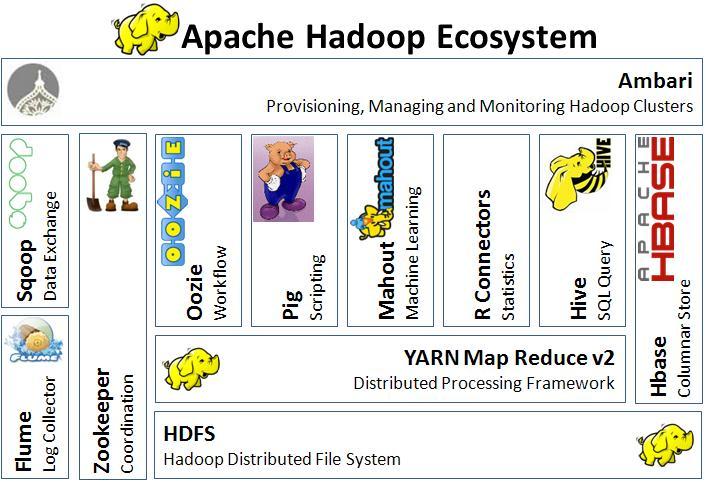
\includegraphics[width=\linewidth]{eco.jpg}
  \caption{Hadoop Ecosystem}
  \label{fig:hadoopecosystem}
\end{figure}

\subsection{Hadoop Core System}
The Apache Hadoop software library is a framework that allows for the distributed processing of large data sets across clusters of computers using simple programming models. It is designed to scale up from single servers to thousands of machines, each offering local computation and storage. Rather than rely on hardware to deliver high-availability, the library itself is designed to detect and handle failures at the application layer, so delivering a highly-available service on top of a cluster of computers, each of which may be prone to failures.

\subsubsection{HDFS\texttrademark}
The Hadoop Distributed File System (HDFS) is a distributed file system designed to run on commodity hardware. It has many similarities with existing distributed file systems. However, the differences from other distributed file systems are significant. HDFS is highly fault-tolerant and is designed to be deployed on low-cost hardware. HDFS provides high throughput access to application data and is suitable for applications that have large data sets. \fullcite{shvachko2010hadoop}


\begin{figure}
  \centering
  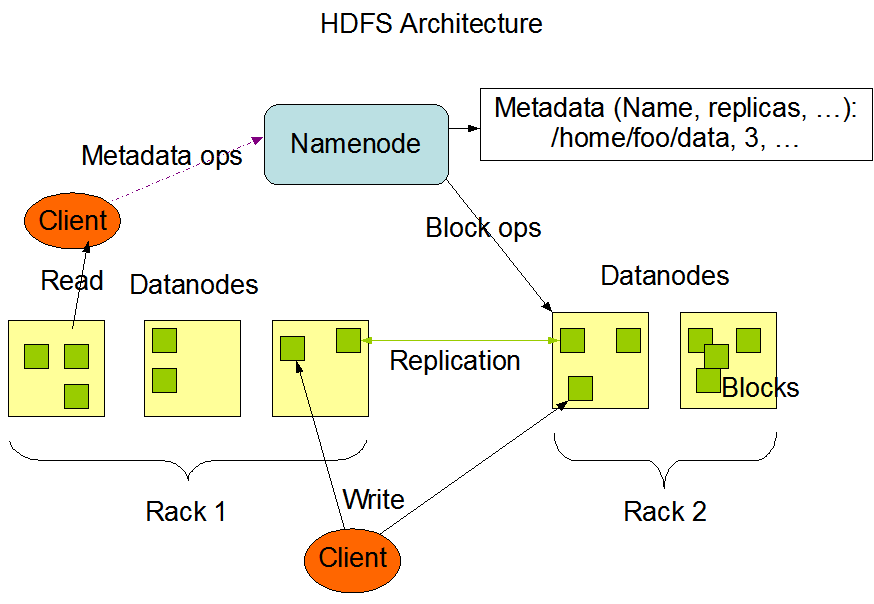
\includegraphics[width=\linewidth]{hdfsarchitecture.png}
  \caption{HDFS Architecture}
\end{figure}

\subsubsection{YARN and MapReduce}
YARN is Hadoop job scheduling system for parallel processing of large data sets using MapReduce. see Figure \ref{fig:mr} 

\begin{figure}
  \centering
  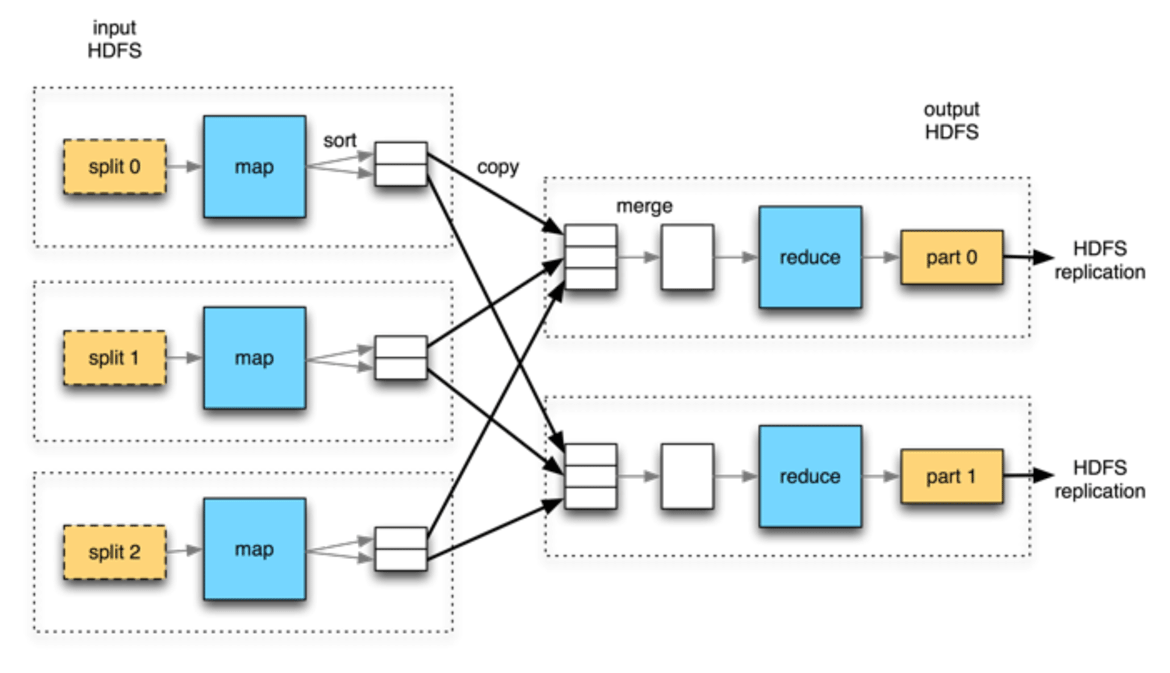
\includegraphics[width=\linewidth]{hadoopfig2.png}
  \caption{MapReduce}
  \label{fig:mr}
\end{figure}

\subsection{Data Access}
OOzie, Pig, Mahaut, R and Hive are developed running on Yarn while HBase access data directly off HDFS.

\subsection{Operation Management}
Tools like Zookeeper, Flume, Sqoop and Ambari are developed for deployment, configuration, diagnostics, and reporting. 

\section{Big Data and Analytics Problem}
\subsection{Batch Processing}
\subsection{Near Realtime Processing}
\subsection{Realtime Processing}

\section{IT Operation Challenges}

\section{Conclusion}

\section{Future Work}

\bibliographystyle{apacite}
\bibliography{\jobname}
\end{document}  